% Hier werden nun einige häufig verwendete Inhaltselemente vorgestellt.

\chapter{Komplexe Inhaltselemente}

\section{Punktliste}

\begin{itemize}
  \item Hamlet
  \item Romeo und Julia
  \item Julius Cäsar
\end{itemize}

\section{Geordnete Liste}

\begin{enumerate}
  \item Hamlet
  \item Romeo und Julia
  \item Julius Cäsar
\end{enumerate}

\section{Definitionsliste}

\begin{description}
  \item [Hamlet] Die Szene ist in Helsingör, nur in der vierten Szene des
  vierten Aktes eine Ebene in Dänemark.
  \item [Romeo und Julia] Die Szene ist im Anfang des fünften Aufzugs in
  Mantua, und sonst immer in Verona.
  \item [Julius Cäsar] Rom, das Lager der Verschwörer nahe Sardis und die Ebenen
  von Philippi.
\end{description}

\section{Geschachtelte Liste}

\begin{enumerate}
\item Hamlet
  \begin{itemize}
  \item König
  \item Ophelia
  \item Hamlet
  \end{itemize}
\item Romeo und Julia
\item Julius Cäsar
\end{enumerate}

\section{Tabellen}

% htb steht für "here", "top" und "bottom" und weist LaTeX an, die Tabelle genau
% hier (falls möglich), zu Beginn oder am Ende der Seite zu setzen.
\begin{table}[htb]
  \caption{Die Werke des \WS}
  % l = linksbündige, c = zentrierte und r = rechtsbündige Spalte. Die Pipe "|"
  % definiert die vertikalen Rahmen der Tabelle.
  \begin{tabular}{|l|c|r|}
    % Die horizontalen Rahmen müssen jeweils manuell eingefügt werden.
    \hline
    % "&" trennt die Spalten einer Zeile.
    \textbf{Werk} & \textbf{Autor} & \textbf{Rollen}\\
    \hline
    Hamlet & \WS & Hamlet, Ophelia, König\\
    \hline
    Julius Cäsar & \WS & Julius Cäsar, Brutus\\
    \hline
    Romeo und Julia & \WS & Romeo, Julia\\
    \hline
  \end{tabular}
\end{table}

\newpage

\section{Abbildungen}

% htb s.o.
\begin{figure}[htb]
\caption{Portrait von \WS}
% Gewisse einfache Manipulationen an Bildern können direkt angegeben werden,
% hier z.B. eine Verkleinerung.
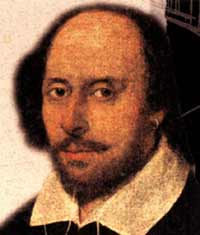
\includegraphics[scale=0.5]{Bilder/Shakespeare.jpg}
\end{figure}

% Vektorgrafiken (z.B. PDF) sollten aufgrund der besseren Skalierbarkeit immer
% bevorzugt werden. Hier zum Vergleich eine Rastergrafik und eine Vektorgrafik.
\begin{figure}[htb]
\caption{Logo der ALTE OLDENBURGER (Bitmap, pixelig bei Vergrößerung)}

\includegraphics[scale=0.3]{Bilder/LogoAO.jpg}
\end{figure}
\begin{figure}[htb]
\caption{Logo der ALTE OLDENBURGER (Vektor, ohne Qualitätsverlust skalierbar)}

\includegraphics[scale=0.8]{Bilder/LogoAO.pdf}
\end{figure}

\section{Mathematische Formeln}

Eine Formel mitten im Fließtext ist $y=mx+b$ und hier geht es weiter.

Lange Formeln werden geklammert:
\( \int\limits_a^b {\frac{d}{dx}F(x)dx} = F(b)-F(a) \)

Und viele Formeln mit Nummerierung erzeugt man mit equation:
\begin{equation}
e=mc^2
\end{equation}

\begin{equation}
u(x,t)= 8 \frac{k_{1}^{2}e^{\alpha_{1}} + k_{2}^{2}e^{\alpha_{2}} + (k_{1}-k_{2})^{2}e^{(\alpha_{1}+ \alpha_{2})} \left[2 + \frac{1}{(k_{1} + k_{2})^{2}} ( k_{1}^{2}e^{\alpha_{1}} + k_{2}^{2}e^{\alpha_{2}}) \right]}{\left[1+e^{\alpha_{1}} + e^{\alpha_{2}} + \left(\frac{k_{1} - k_{2}}{k_{1}+k_{2}} \right)^{2} e^{\alpha_{1}+ \alpha_{2}} \right]^{2}}
\end{equation}

\section{URLs}
\url{http://blog.stefan-macke.com}